% Enable warnings about problematic code
\RequirePackage[l2tabu, orthodox]{nag}

\documentclass{WeSTassignment}

% The lecture title, e.g. "Web Information Retrieval".
\lecture{Introduction to Web Science}
% The names of the lecturer and the instructor(s)
\author{%
  Prof. Dr.~Steffen~Staab\\{\normalsize\mailto{staab@uni-koblenz.de}} \and
  Ren{\'e}~Pickhardt\\{\normalsize\mailto{rpickhardt@uni-koblenz.de}} \and
   Korok~Sengupta\\{\normalsize\mailto{koroksengupta@uni-koblenz.de}}
}
% Assignment number.
\assignmentnumber{3}
% Institute of lecture.
\institute{%
  Institute of Web Science and Technologies\\%
  Department of Computer Science\\%
  University of Luxembourg%
}
% Date until students should submit their solutions.
\datesubmission{November 16, 2016, 10:00 a.m.}
% Date on which the assignments will be discussed in the tutorial.
\datetutorial{November 18, 2016, 12:00 p.m.}

% Set langauge of text.
\setdefaultlanguage[
  variant = american, % Use American instead of Britsh English.
]{english}

% Specify bib file location.
\addbibresource{bibliography.bib}

% For left aligned centerd boxes
% see http://tex.stackexchange.com/a/25591/75225
\usepackage{varwidth}

% ==============================================================================
% Document

\begin{document}

\maketitle

The main objective of this assignment is for you understand different concepts that are associated with the "Web". In this assignment we cover two topics: 1) DNS \& 2) Internet. 

These tasks are not always specific to \enquote{Introduction to Web Science}.
For all the assignment questions that require you to write a code, make sure to include the code in the answer sheet, along with a separate python file. Where screen shots are required, please add them in the answers directly and not as separate files.\\ \\ 

%Please mention your team Names here: 
Team Name: Echo \\
Team Members: Hanadi Tamimi, Keya Kashem, Md Jakaria Nawaz

% ------------------------------------------------------------------------------

\section{DIG Deeper (5 Points)}

Assignment 1 started with you googling certain basic tools and one of them was "\emph{dig}". 
\begin{enumerate}
\item Now using that dig command, find the IP address of \url{ www.uni-koblenz-landau.de}
\item In the result, you will find "SOA". What is SOA? 
\item Copy the SOA record that you find in your answer sheet and explain each of the components of SOA with regards to your find. Merely integrating answers from the internet wont fetch you points.  

\end{enumerate}
Try the experiment once from University network and once from Home network and see if you can find any differences and if so, clarify why. 

\textbf{Answers:}\\
(1) IP Address for www.uni-kobelenz-landau.de is 141.26.200.8 \\
The result is same for both network. \\
Network 1 \\
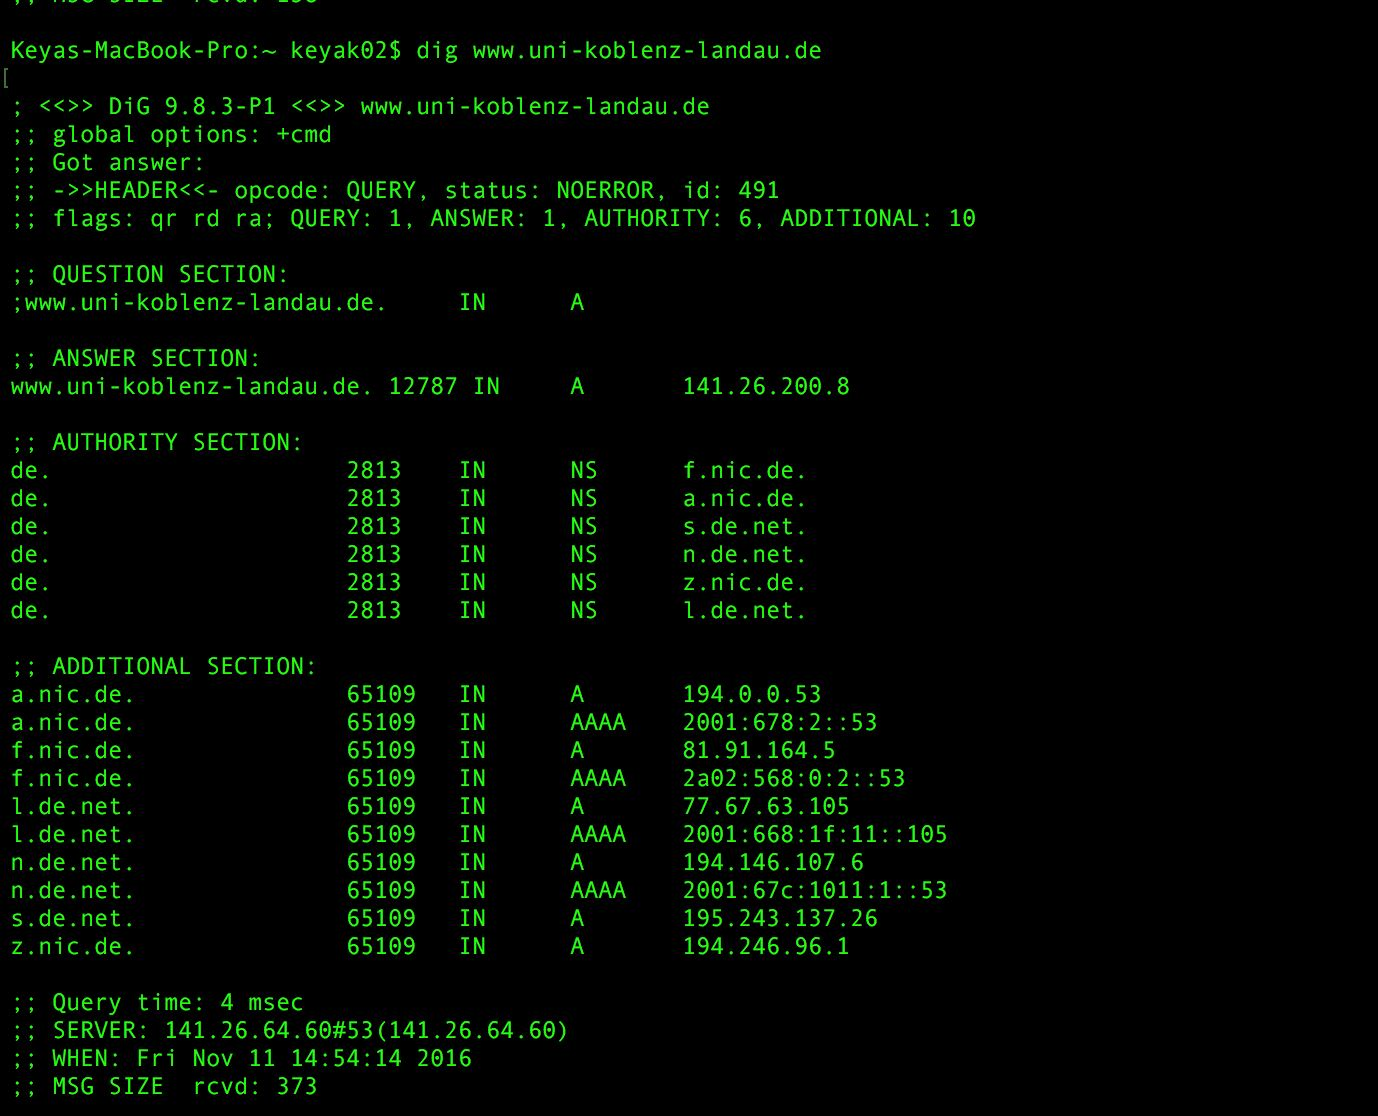
\includegraphics[width=1\textwidth]{images/net-com1.png} \\ \\ \\
Network 2 \\
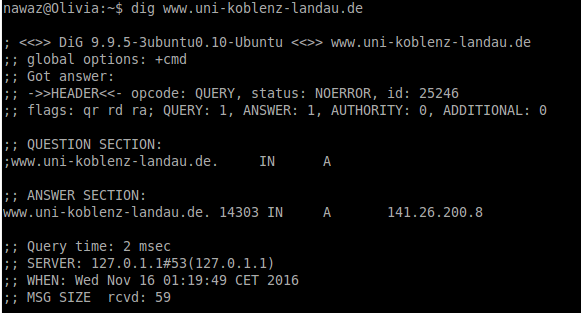
\includegraphics[width=1\textwidth]{images/net2-com1.png} \\ \\
(2) SOA: The full form of SOA is Start Of Authority. An SOA record is a Start of Authority. Every domain must have a Start of Authority record at the cutover point where the domain is delegated from its parent domain. It is an important component of a zone file in Domain Name System (DNS). An SOA record contains important information for the management of the zone, in particular the zone transfer.The SOA record consists of 7 fields. \\
Network 1 \\
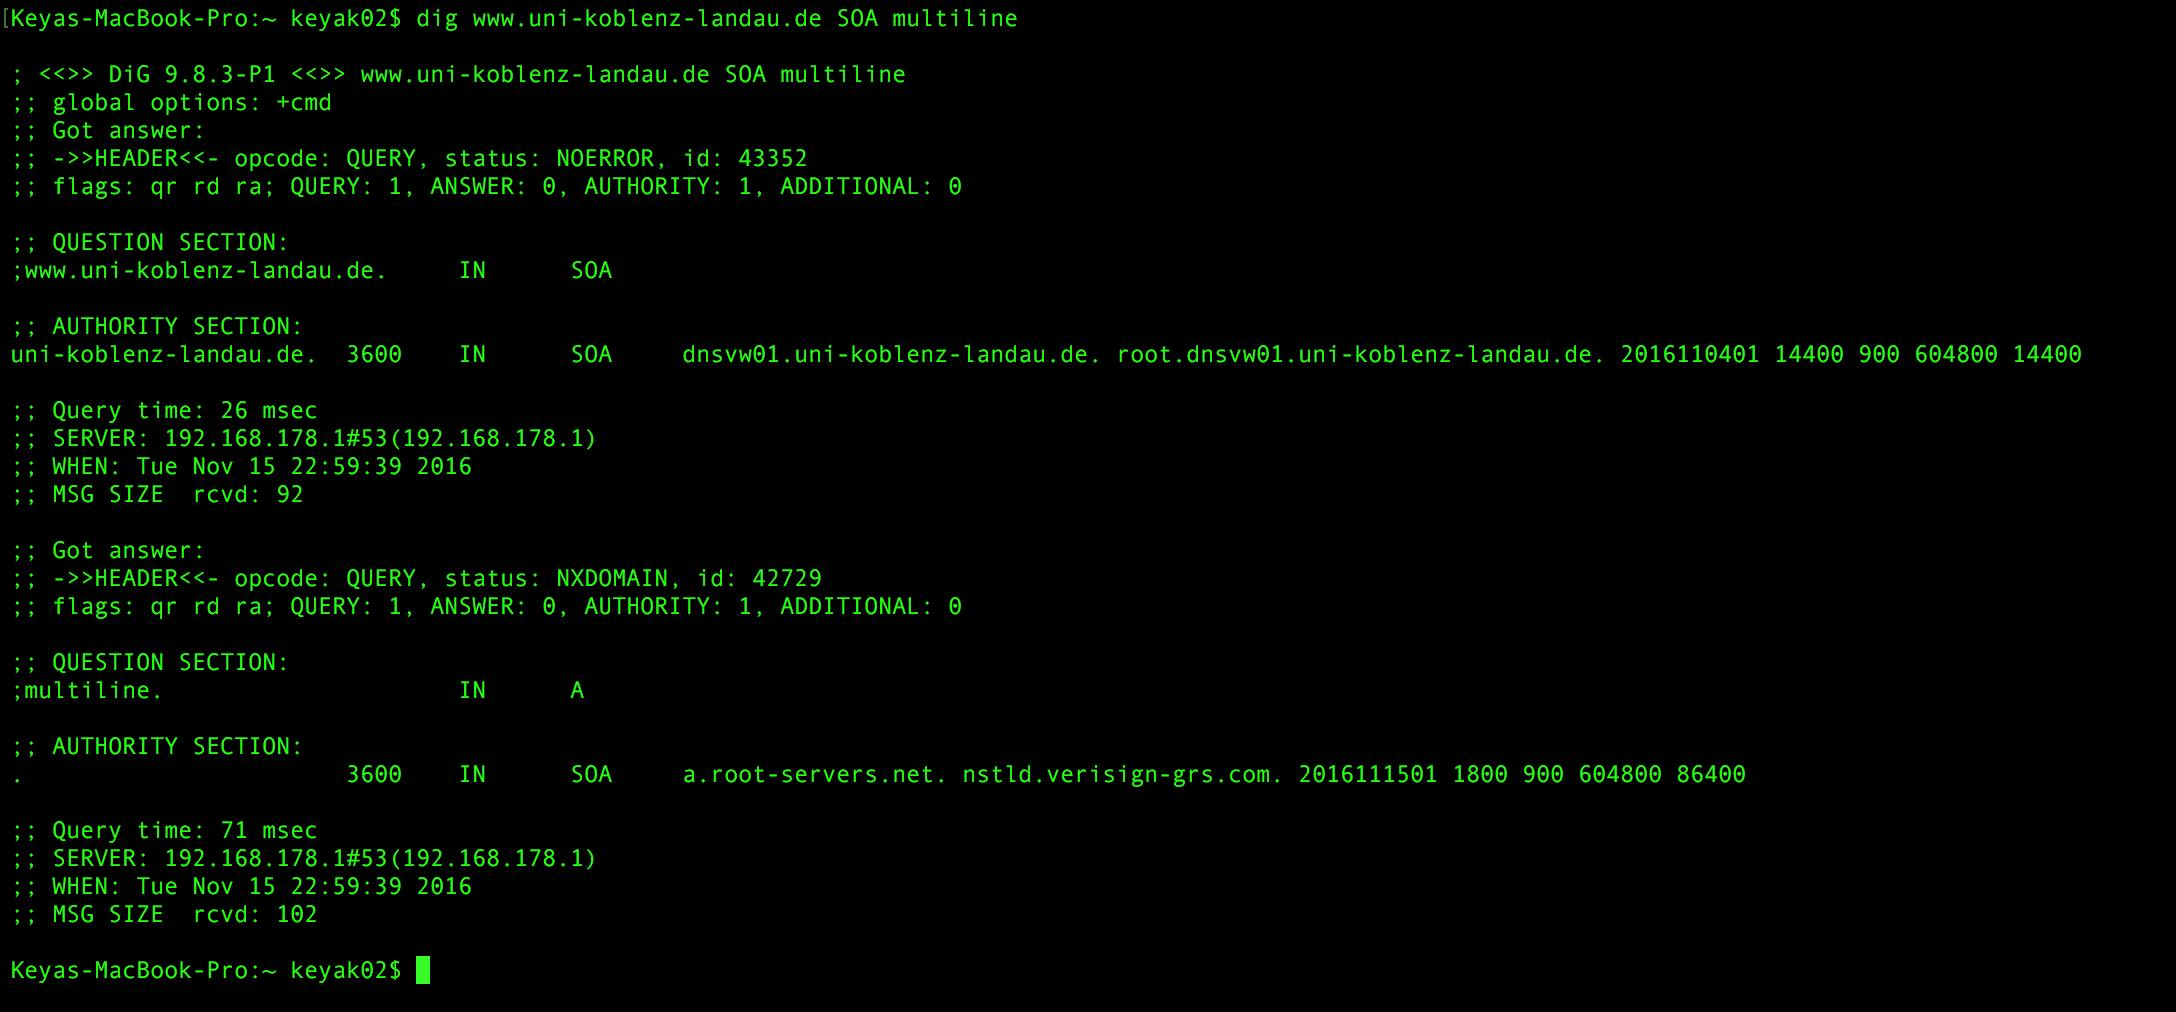
\includegraphics[width=1\textwidth]{images/net-com2.png} \\ \\ \\ \\
Network 2 \\
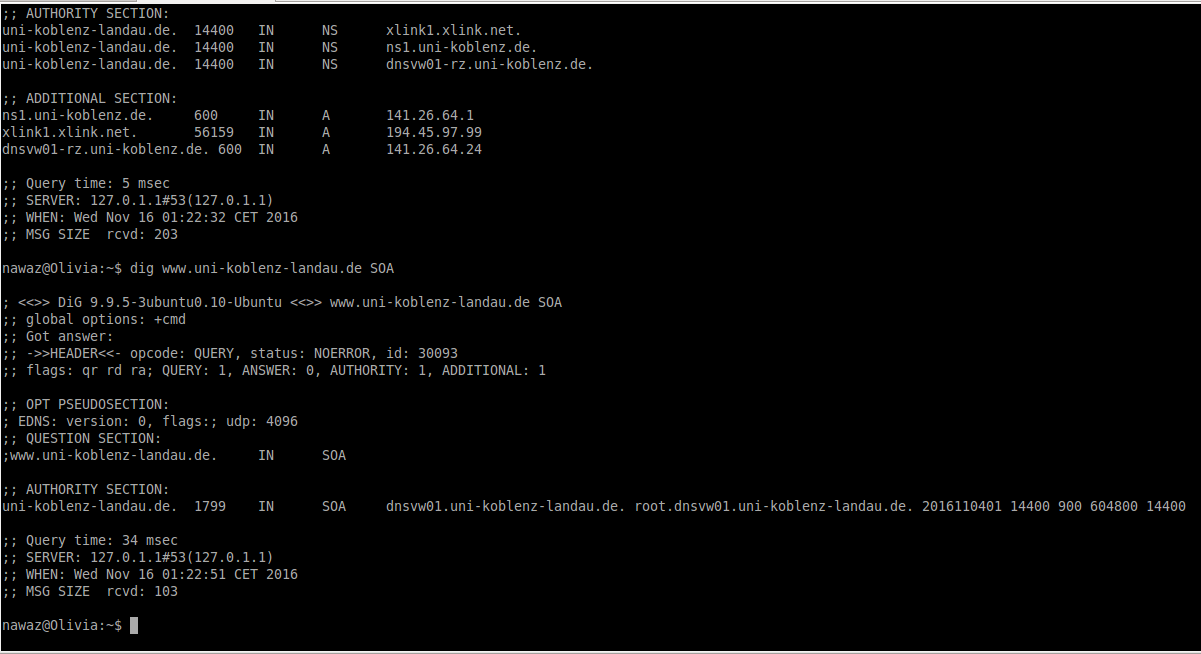
\includegraphics[width=1\textwidth]{images/net2-com2.png} \\ \\
(3) The SOA record of www.uni-koblenz-landau.de is described below- \\
\begin{itemize}
	\item Primary- The primary name server for the domain - dnsvw01.uni-koblenz-landau.de \\
	\item Mail address - The responsible party for the domain - root.dnsvw01.uni-koblenz-landau.de \\
	\item serial number- A timestamp that changes whenever the domain is updated - 2016110401 \\
	\item Refresh - The number of seconds before the zone should be refreshed - 14400 \\
	\item Retry - The number of seconds before a failed refresh should be retried - 900 \\
	\item Expire - The upper limit in seconds before a zone is considered no longer authoritative - 604800 \\
	\item TTL -How long a resolver should consider a negative result for a subdomain to be valid before retrying - 14400 \\
\end{itemize}
% ------------------------------------------------------------------------------

\section{Exploring DNS (10 Points)}

In the first part of this assignment you were asked to develop a simple TCP Client Server. Now, using \textbf{that} client server setup.
This time a url should be send to the server and the server will split the url into the following:\\ 

\url{http://www.example.com:80/path/to/myfile.html?key1=value1&key2=value2#InTheDocument}

\begin{enumerate}
\item Protocol
\item Domain
\item Sub-Domain
\item Port number
\item Path
\item Parameters
\item Fragment
\end{enumerate}

The Protocol for sending the URL will be a string terminated with \backslash r \backslash n.

P.S.: You are \textbf{not} allowed to use libraries like \texttt{urlparse} for this question. You will also not use "Regular Expressions" for this. 

\textbf{Answer:} 
Code (client.py): \\ 
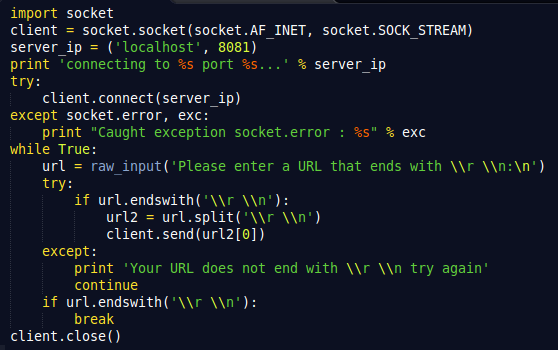
\includegraphics[width=1\textwidth]{images/client-image.png} \\
Git link (client.py): \\
{\color{blue}\underline{\href{https://github.com/jakaria-nawaz/Echo/blob/master/Echo/assignment3/client.py/}{https://github.com/jakaria-nawaz/Echo/blob/master/Echo/assignment3/client.py/}}} \\ \\
Code (server.py): \\ 
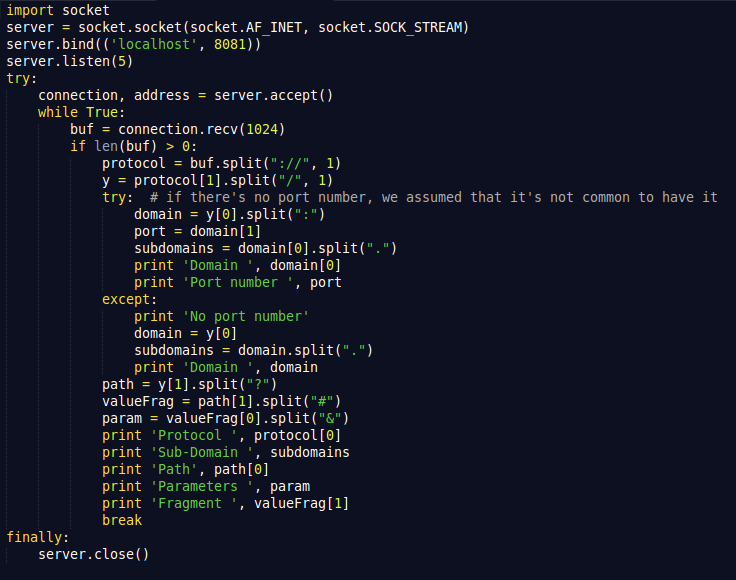
\includegraphics[width=1\textwidth]{images/server-image.png} \\
Git link (server.py): \\
{\color{blue}\underline{\href{https://github.com/jakaria-nawaz/Echo/blob/master/Echo/assignment3/server.py/}{https://github.com/jakaria-nawaz/Echo/blob/master/Echo/assignment3/server.py/}}} \\ \\
Result(Screenshot): \\
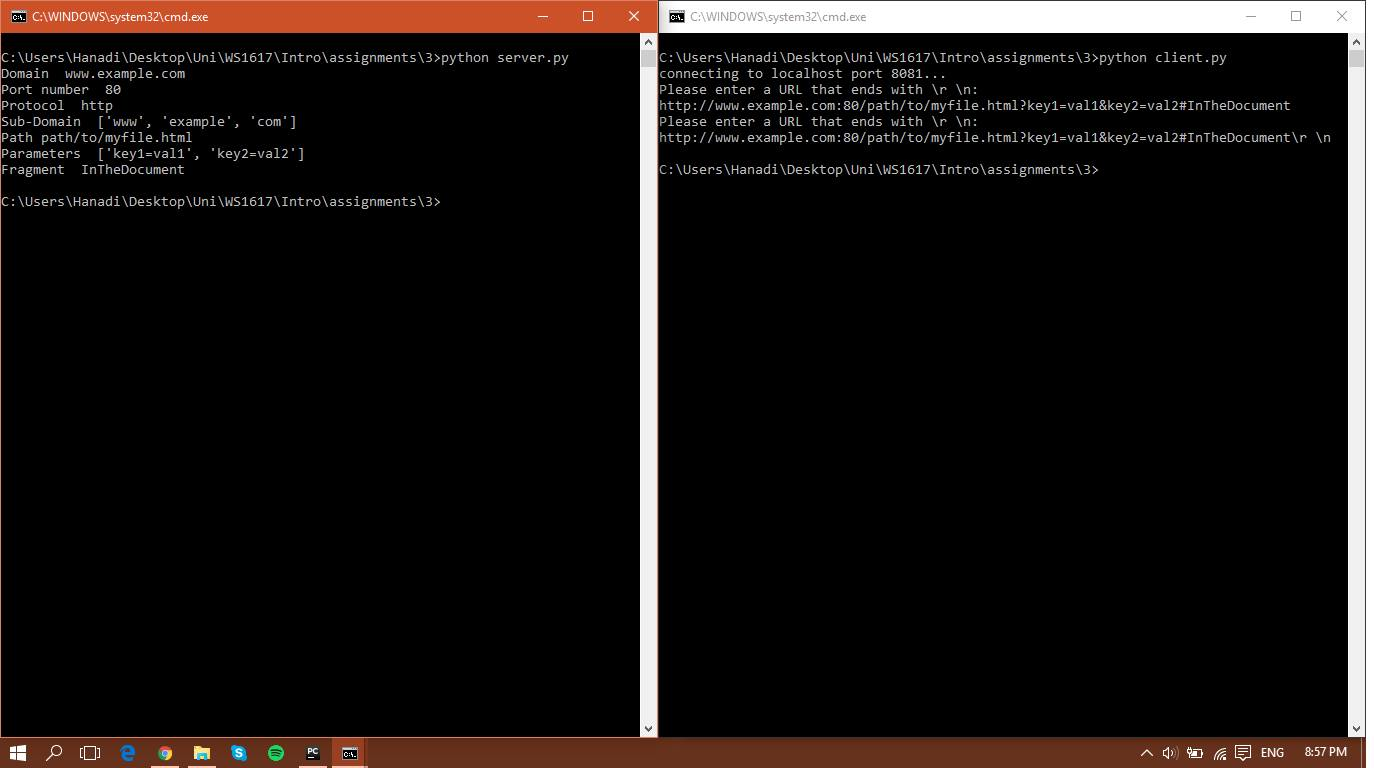
\includegraphics[width=1\textwidth]{images/python-result-cmd.png} \\

% ------------------------------------------------------------------------------


\section{DNS Recursive Query Resolving (5 Points)}

You have solved the "Routing Table" question in Assignment 2. We updated the routing tables once more. resulting in the following tables creating the following topology 

% Please add the following required packages to your document preamble:
% \usepackage[normalem]{ulem}
% \useunder{\uline}{\ul}{}
\begin{table}[h]
\centering
\caption{Routing Table}
\label{routing table}
\scalebox{0.8}{
\begin{tabular}{|c|c|c|c|c|c|c|c|c|c|c|}
\hline
\multicolumn{3}{|c|}{\textbf{Router1}} &        & \multicolumn{3}{c|}{\textbf{Router2}} &        & \multicolumn{3}{c|}{\textbf{Router3}} \\ \hline
Destination  & Next Hop    & Interface &        & Destination & Next Hop    & Interface &        & Destination  & Next Hop   & Interface \\ \hline
67.0.0.0     & 67.68.3.1   & eth 0     &        & 205.30.7.0  & 205.30.7.1  & eth 0     &        & 205.30.7.0   & 205.30.7.2 & eth 0     \\ \hline
62.0.0.0     & 62.4.31.7   & eth 1     &        & 156.3.0.0   & 156.3.0.6   & eth 1     &        & 88.0.0.0     & 88.6.32.1  & eth 1     \\ \hline
88.0.0.0     & 88.4.32.6   & eth 2     &        & 26.0.0.0    & 26.3.2.1    & eth 2     &        & 25.0.0.0     & 25.03.1.2  & eth 2     \\ \hline
141.71.0.0   & 141.71.20.1 & eth 3     &        & 141.71.0.0  & 141.71.26.3 & eth 3     &        & 121.0.0.0    & 121.0.3.1  & eth 3     \\ \hline
26.0.0.0     & 141.71.26.3 & eth3      &        & 67.0.0.0    & 141.71.20.1 & eth 3     &        & 156.3.0.0    & 205.30.7.1 & eth 0     \\ \hline
156.3.0.0    & 88.6.32.1   & eth 2     &        & 62.0.0.0    & 141.71.20.1 & eth 3     &        & 26.0.0.0     & 205.30.7.1 & eth 0     \\ \hline
205.30.7.0   & 141.71.26.3 & eth 3     &        & 88.0.0.0    & 141.71.20.1 & eth 3     &        & 141.71.0.0   & 205.30.7.1 & eth 0     \\ \hline
25.0.0.0     & 88.6.32.1   & eth 2     &        & 25.0.0.0    & 205.30.7.2  & eth 0     &        & 67.0.0.0     & 88.4.32.6  & eth 1     \\ \hline
121.0.0.0    & 88.6.32.1   & eth 2     &        & 121.0.0.0   & 205.30.7.2  & eth 0     &        & 62.0.0.0     & 88.4.32.6  & eth 1     \\ \hline
\end{tabular}
}
\end{table}

\begin{figure}[h]
  \centering
  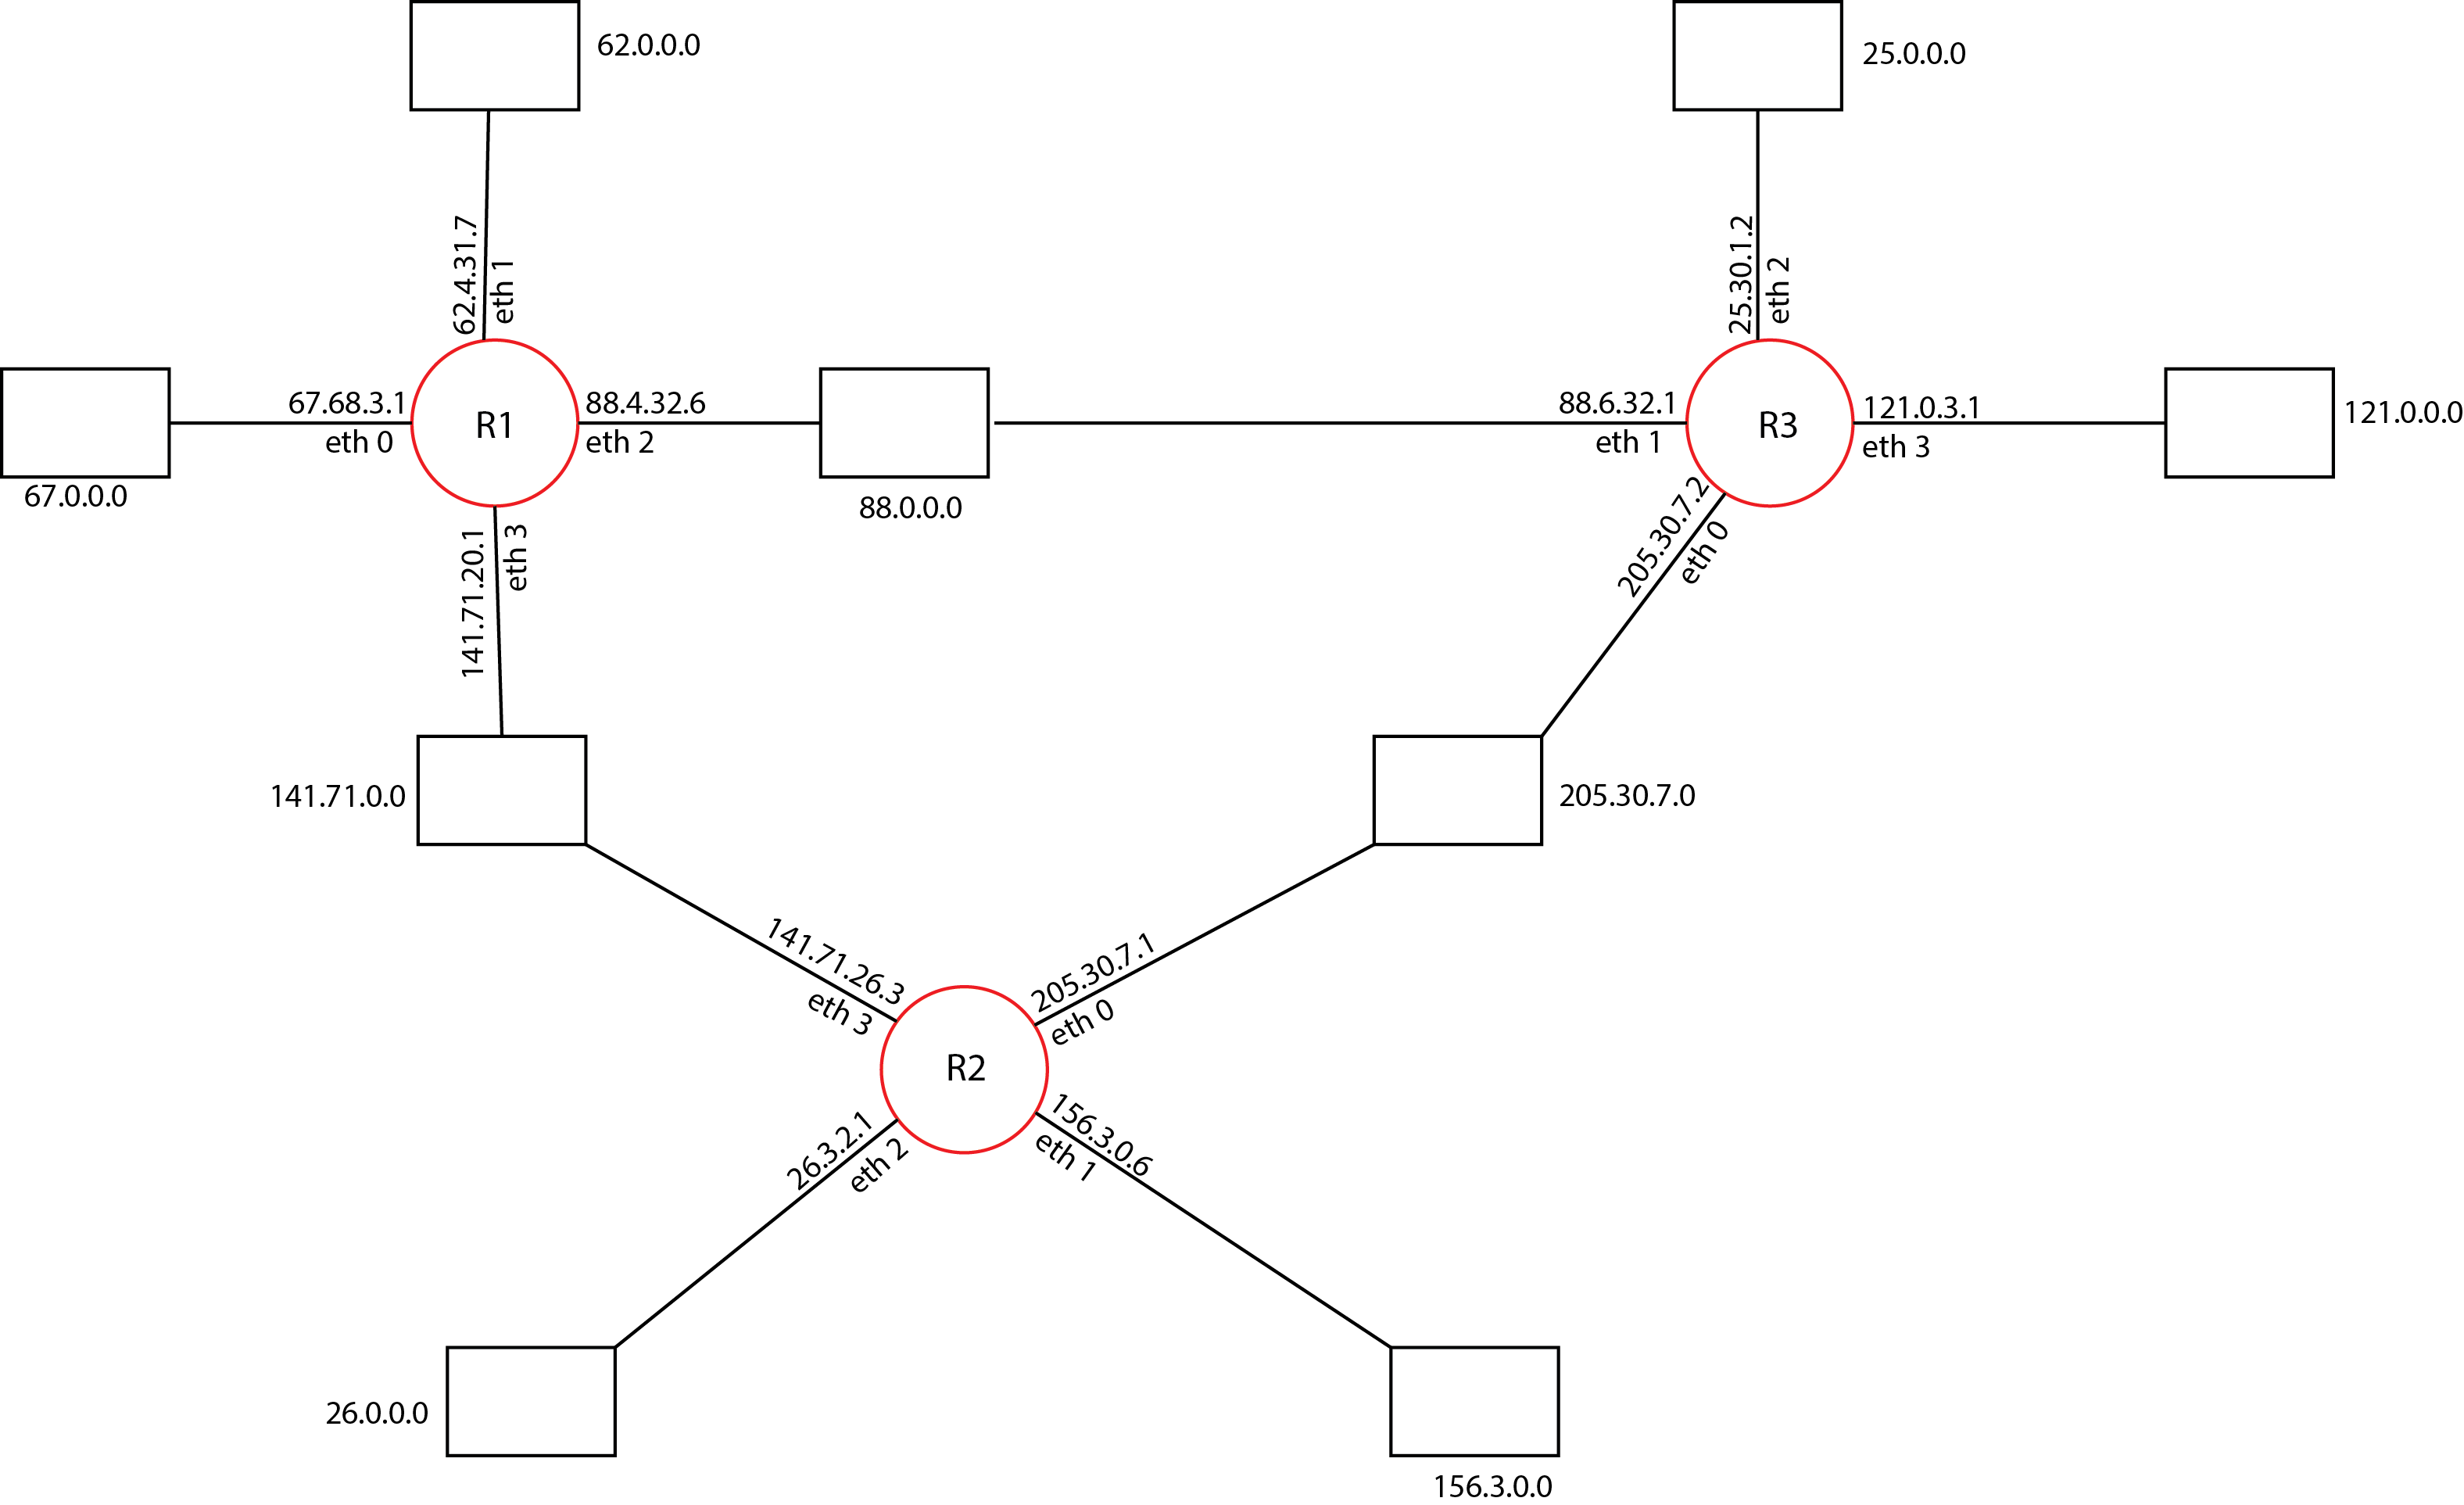
\includegraphics[scale=0.45]{ass3_DNS.png}
   \caption{DNS Routing Network}
     \label{fig:routing} 
\end{figure}

Let us asume a client with the following ip address 67.4.5.2 wants to resolve the following domain  \texttt{subdomain.webscienceexampledomain.com} using the DNS.

You can further assume the root name server has the IP address of 25.8.2.1 and the name-server for \texttt{webscienceexampledomain.com} has the IP address 156.3.20.2. 
Finally the sub-domain is handled by a name server with the IP of 26.155.36.7. 

Please explain how the traffic flows through the network in order to resolve the recursive DNS query. You can assume ARP tables are cached so that no ARP-requests have to be made. 

\textbf{Hint: You can start like this}: 

67.4.5.2 creates an IP packet with the source address XXXXXX an destination address YYYYY inside there is the DNS request. This IP packet is send as an ethernet frame to ZZZZZ. 
ZZZZZ receives the frame and forwards the encapsulated IP packet to ....

Also you can assume the DNS requests and responses will fit inside one IP packet. You also don't have to write down the specific DNS requests and responses in hex. \\ \\

\textbf{Answer:} \\
In this solution we have followed what was explained in the video of "DNS address resolution" and mixed it with the routing table algorithm that we learnt in previous weeks. \\
Therefore, we are assuming that (Router1), which is resposible for the network that the client is connected to, to be the ISP. \\
The ISP is going to send all the requests and receive them until it receives the final correct response then sends it to the client. \\ 
Moreover, we are assuming (Router2) and (Router3) to be DNS servers. \\
We are also assuming that "webscienceexampledomain" and "com" is in a zone (Zone2) with the "subdomain", and that zone is considered to be handled by (Router2); since (Router2) is responsible for both of them according to the routing tables. \\
Also, there's another assumed zone (Zone1 that includes the "root server" and the ".com" domain which is handled by (Router3). We added ".com" in the zone to make it overlap with the whole scenario. Since the question also hasn't given us an IP for the .com domain. \\ \\

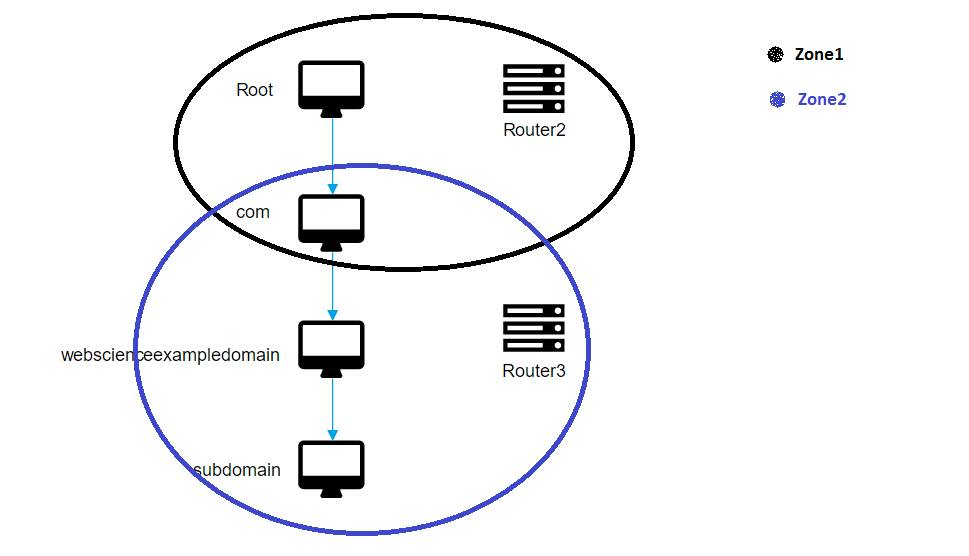
\includegraphics[width=1\textwidth]{images/zones-dns.png} \\ \\ \\

As client 67.4.5.2 wants to resolve the domain "subdomain.webscienceexampledomain.com" using DNS. First, the client will issue a request to the ISP, asking for the address of the domain "subdomain.webscienceexampledomain.com". \\
The ISP will forward that request to the root server with IP 25.8.2.1 that exists under (Router3). (Router3) as a DNS will know that it doesn't have that domain in its networks. Therefore it will send back a response to the ISP, in that response will be the IP address of the DNS that the ISP should send the request to, which is now 156.3.20.2 \\
The ISP sends a request to the "webscienceexampledomain.com" with the IP 156.3.20.2, which is under (Router2). (Router2) as a DNS will be asked for the address of the domain "subdomain.webscienceexampledomain.com". (Router2) (DNS) knows that this domain lies in its network and therefore is able to resolve its IP address. (Router2) will send back a response to the ISP with the IP address of the requested domain. \\
The ISP sends back a response to the client 67.4.5.2 with the IP address of the domain "subdomain.webscienceexampledomain.com" \\
There is another description given hop by hop means how the request will travel, which hop after which hop. It is uploaded in the git as text file.\\ Here is the link: \\
{\color{blue}\underline{\href{https://github.com/jakaria-nawaz/Echo/blob/master/Echo/assignment3/hop-description(quses3).txt/}{https://github.com/jakaria-nawaz/Echo/blob/master/Echo/assignment3/hop-description(quses3).txt/}}}

% ------------------------------------------------------------------------------




\makefooter

\end{document}
